\documentclass[a4paper,11pt]{article}

\usepackage[T1]{fontenc}
\usepackage[french]{babel}
\usepackage[utf8x]{inputenc}
%\usepackage{palatino} %change la police d'écriture.
\usepackage{lipsum} %pour avoir un texte, en latin, déja écrit, inutile dans 99,999999 % du temps.


%modules mathématiques :
\usepackage{amsmath}
\usepackage{amssymb}
\usepackage{mathrsfs} %pour avoir un police d'écriture anglo-saxonne en mode mathématique.
\usepackage{amsthm}
\usepackage{amssymb} %symboles en plus.
\usepackage{amsfonts}
\usepackage{a4wide}
%autres packages :
\usepackage{verbatim} %pour pouvoir changer de police dans le document.
\usepackage{mathptmx} %pour utiliser une autre police
\usepackage{dsfont}
\usepackage{graphicx} %pour pouvoir faire des graphes.
\usepackage{color} %pour mettre de la couleur
\definecolor{bblack}{cmyk}{0,0,0,1} 
\usepackage[colorlinks=true,linkcolor = black,urlcolor=black]{hyperref} %pour les liens hypertextes
% \usepackage{Sweave} %pour du code R
% \usepackage{mhchem}
%si on veut mettre du code python
\usepackage{listings}
\definecolor{dkgreen}{rgb}{0,0.4,0}
\definecolor{gray}{rgb}{0.5,0.5,0.5}
\definecolor{mauve}{rgb}{0.58,0,0.82}
\definecolor{dkyellow}{cmyk}{0, 0, 0.2, 0}
\lstset{
  language=Python,                % the language of the code
  basicstyle= \footnotesize,      % the size of the fonts that are used for the code
  numbers=left,                   % where to put the line-numbers
  numberstyle=\tiny\color{gray},  % the style that is used for the line-numbers
  stepnumber=2,                   % the step between two line-numbers. If it's 1, each line 
                                  % will be numbered
  showspaces=false,               % show spaces adding particular underscores
  showtabs=false,                 % show tabs within strings adding particular underscores
  frame=single,                   % adds a frame around the code
  rulecolor=\color{black},        % if not set, the frame-color may be changed on line-breaks within not-black text (e.g. commens (green here))
  tabsize=2,                      % sets default tabsize to 2 spaces
  captionpos=b,                   % sets the caption-position to bottom
  breaklines=true,                % sets automatic line breaking
  breakatwhitespace=false,        % sets if automatic breaks should only happen at whitespace
  keywordstyle=\color{blue},      % keyword style
  commentstyle=\color{dkgreen},   % comment style
  stringstyle=\color{mauve},       % string literal style
  backgroundcolor=\color{dkyellow},      % choose the background color. You must add \usepackage{color}
}
%%%%%%%%%%%%%%%%%%%%%%%%%%%

%%%%%% Pour reduire les marges ! %%%%%%%%%%%%%%%
%\setlength{\textwidth}{15cm} %Largeur du texte : n
%\setlength{\marginparwidth}{0cm}
%\setlength{\oddsidemargin}{0.5cm} %m avec 2m+n = 16 pour que ca marche bien.
%\setlength{\headheight}{0cm}
%\setlength{\topmargin}{2cm} %hauteur marge d'en haut
%\setlength{\headsep}{0cm} %hauteur de l'en tete
%\setlength{\textheight}{21cm} %hauteur du texte
%\setlength{\footskip}{0cm} %hauteur du pied de page
%\setlength{\marginparsep}{0cm}
%%%%%% Commandes pour structurer le texte %%%%%%%
%\part
%\section
%\subsection
%\subsubsection

%Pour énumérer, dans une section ou une sous-section :
%\begin{enumerate}
%\item texte
%\item texte2 etc.
%\end{enumerate}

%\vspace{n pt} : met un espace de n point(s) entre les paragraphes. Attention à l'utilisation.
%\vspace{6 ex} : met un espace de 6 hauteurs de police entre les paragraphes. Attention à l'utilisation.
%\vspace*{...} : force l'espace, même si c'est au début ou à la fin d'une page. Tres attention a l'utilisation.

% \\ pour passer une ligne
% \newpage pour écrire ce qui suit sur une nouvelle page
% \clearpage : pour ne rien ecrire de plus sur la page en cours

%%%%%%%%%%%%%%%%%%%%%%%%%%%%%%%%%%%%%%%%%%%%%%%%%%

%%%%%%%%%%%%% Deux modes maths %%%%%%%%%%%%%%%%%%%
% mettre entre $, ex : $ 2+2 = 4$ 
% mettre entre \[ \], ex : \[ 2+2 = 4 \].
%Attention, rendus différents
%%%%%%%%%%%%%%%%%%%%%%%%%%%%%%%%%%%%%%%%%%%%%%%%%%

%%%%%%%%%%%%Pour faire un calcul, centré sur les = %%%%%%%%%%%%%%%
%\begin{align*}
%calcul, tout sera déja en mode maths.
%a &= b
%&= c+d-E etc.
%\end{align*}
%%%%%%%%%%%%%%%%%%%%%%%%%%%%%%%%%%%%%%%%%%%%%%%%%%



%%%%%%%%%%%% Pour mettre en valeur un résultat %%%%%%%%%%%%%%%%%%%
%\begin{abstract}
 %résultat\begin{abstract}
%\end{abstract}
% Attention au rendu, il faudrait réussir à enlever la phrase en gras juste au dessus.
%%%%%%%%%%%%%%%%%%%%%%%%%%%%%%%%%%%%%%%%%%%%%%%%%%%%%%%%%%%%%%%%%%%

%%%%%%%%%%%% Pour des références %%%%%%%%%%%%%%%%%%%%
%\label{ref1}
%\ref{ref1}
%\pageref{ref1}
%%%%%%%%%%%%%%%%%%%%%%%%%%%%%%%%%%%%%%%%%%%%%%%%%%%%%

%%%%%%%%%%%% Pour des fleches stylees %%%%%%%%%%%%%%%
%\xrightarrow[nce qu'il y aura en dessous]{ce qu'il y aura au dessus}
%ex :\xrightarrow[n \to \infty]{P-ps}
%%%%%%%%%%%%%%%%%%%%%%%%%%%%%%%%%%%%%%%%%%%%%%%%%%%%%


%%%%%%%%%%% Pour rajouter des trucs en dessous (au dessus d'une expression) %%%%%%%%%%%%%%%%%%
%\underset{ce qu'il y a en dessous}{ce qu'il y a au dessus}
%\underset{n\to \infty}{=}

%\overset{ce qu'il y a au dessus}{ce qu'il y a en dessous}
%\overset{n\to \infty}{=}
%%%%%%%%%%%%%%%%%%%%%%%%%%%%%%%%%%%%%%%%%%%%%%%%%%%%%%

%%%%%%%%%%% Pour inclure un graphique %%%%%%%%%%%%%%%%
%\includegraphics[hauteur]{nom de l'image} % L'image doit être dans le même fichier que le fichier.tex.
%ex : \includegraphics[width=11cm]{unif_n10.jpeg}
%%%%%%%%%%%%%%%%%%%%%%%%%%%%%%%%%%%%%%%%%%%%%%%%%%%%%%
                    
                     
% mathbb pour les corps R, C ...
% mathcal pour les lettres caligraphiques (tribus etc.)
% mathfrak pour les lettres ghotiques
% mathbf pour les lettres en gras

%%%%%%%%%%%% Pour le titre la date et autres infos du pdf %%%%%%%%%%%%%
% \title{Book Report on : Heat Wave}
% \author{Benjamin Donnot}
% \date{}

%\pdfinfo{%
%  /Title    ()
%  /Author   ()
%  /Creator  ()
%  /Producer ()
 % /Subject  ()
%  /Keywords ()
%}
%%%%%%%%%%%%%%%%%%%%%%%%%%%%%%%%%%%%%%%%%%%%%%%%%%%%%%%%%%%%%%%%%%%%%%%%%%

%%%%%%%%%%%%%%%%%%%%%%% Affichage du titre ou autre %%%%%%%%%%%%%%%%%%%%%%
% \maketitle : affiche le titre
%%%% \tableofcontents : pour faire une table des matières
%%%%%%%%%%%%%%%%%%%%%%%%%%%%%%%%%%%%%%%%%%%%%%%%%%%%%%%%%%%%%%%%%%%%%%%%%%

%%%%%%%%%%%%Pour des entetes stylees%%%%%%%%%%%%%%%%%%%
\makeatletter
\def\clap#1{\hbox to 0pt{\hss #1\hss}}%
\def\ligne#1{%
\hbox to \hsize{%
\vbox{\centering #1}}}%
\def\haut#1#2#3{%
\hbox to \hsize{%
\rlap{\vtop{\raggedright #1}}%
\hss
\clap{\vtop{\centering #2}}%
\hss
\llap{\vtop{\raggedleft #3}}}}%
\def\bas#1#2#3{%
\hbox to \hsize{%
\rlap{\vbox{\raggedright #1}}%
\hss
\clap{\vbox{\centering #2}}%
\hss
\llap{\vbox{\raggedleft #3}}}}%
\def\maketitle{%
\thispagestyle{empty}\vbox to \vsize{%
\haut{}{\@blurb}{}
\vfill
\vspace{1cm}
\begin{flushleft}
\usefont{OT1}{ptm}{m}{n}
\huge \@title
\end{flushleft}
\par
\hrule height 4pt
\par
\begin{flushright}
\usefont{OT1}{phv}{m}{n}
\Large \@author
\par
\end{flushright}
\vspace{1cm}
\begin{center}
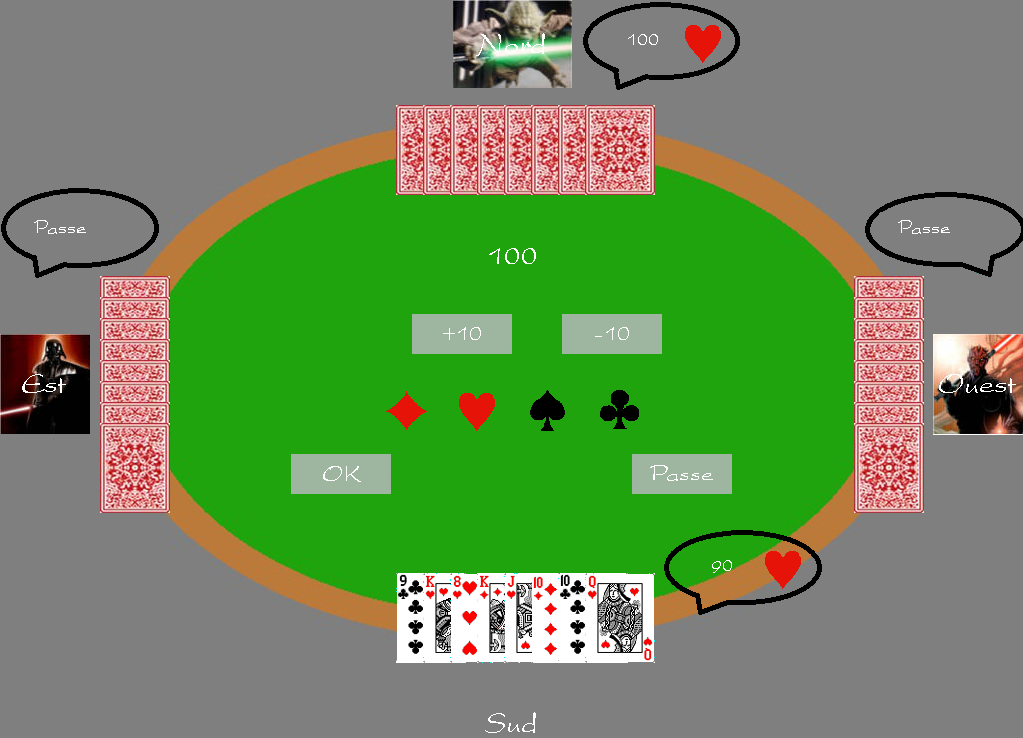
\includegraphics[width=13cm]{img/Coinche.png}
\end{center}

\vfill
\vfill
\bas{}{}{}
}
\cleardoublepage
}
\def\date#1{\def\@date{#1}}
\def\author#1{\def\@author{#1}}
\def\title#1{\def\@title{#1}}
\def\location#1{\def\@location{#1}}
\def\blurb#1{\def\@blurb{#1}}


\date{30 avril 2015}
\title{}
\location{}\blurb{}
\makeatother
\title{Projet Informatique : Jeu de Coinche}
\author{Benjamin DONNOT}
\location{}
\blurb{}

\renewcommand{\thesection}{\Roman{section}}
\renewcommand{\thesubsection}{\Roman{section}.\arabic{subsection}}
\renewcommand{\thesubsubsection}{\Roman{section}.\arabic{subsection}.\roman{subsection}}
%%%%%%%%%Pour l'en-tete et le pied de page%%%%%%%%%%%%%%%%%%
\usepackage{fancyhdr}
\pagestyle{fancy}
\usepackage{lastpage}
\renewcommand\headrulewidth{1pt}
\renewcommand\footrulewidth{1pt}
\fancyfoot[C]{Projet informatique\\ \textbf{Page \thepage/\pageref{LastPage}}}
\fancyfoot[R]{ENSAE 3\ieme{} année \\ Data Science}
\fancyfoot[L]{Benjamin DONNOT }

\begin{document}
\maketitle
\tableofcontents
\clearpage
\section*{Introduction}
\addcontentsline{toc}{section}{Introduction} 
Depuis le cours de python de première année, j'ai découvert un champ assez vaste informatiquement : celui de l'\textit{intelligence artificielle}. Ce terme assez générique a plusieurs sens. Ce que j'entends par "intelligence artificielle" dans tout ce rapport, et plus généralement dans le projet tout entier, c'est la capacité pour un ordinateur à prendre des décisions "cohérentes" et ainsi à jouer "convenablement" à la coinche. \\

La "coinche", comme de nombreux jeu de cartes ne se joue pas en information parfaite : les cartes des adversaires sont cachées ! Résoudre\footnote{Entendre ici : performer aussi bien que les humains en général.} un jeu de coinche pourrait donc permettre de faire des avancées dans certains types de problèmes rencontrés dans la vie de tous les jours qui ne se limitent pas simplement aux jeux de cartes. Chaque jour, nous sommes amenés à prendre des décisions dans un environnement incertains\footnote{Qui est plus nettement plus compliqué que l'environnement simplifié du jeu de Coinche.}. \\
Ainsi, il n'est pas rare que la recherche en intelligence artificielle se concentre sur des jeux. C'était notamment le cas au début des années 90 avec IBM et "Deep Blue", le premier ordinateur à avoir battu un grand maître aux échecs\footnote{Cette victoire a suscité de nombreuses polémiques qui ne seront pas abordées ici, car ce n'est pas le sujet. Toujours est-il qu'aujourd'hui, il est communément admis que les ordinateurs jouent mieux que les humains aux échecs.}. Encore aujourd'hui, de nombreuses compétitions de jeux se voient affronter les meilleurs programmes informatiques du monde, notamment au Go\footnote{On pourra se reporter au "Computer Go" :  \url{http://en.wikipedia.org/wiki/Computer_Go}.}, ou encore le Bridge\footnote{Jeu relativement proche de la Coinche, mais beaucoup plus populaire outre Manche et outre Atlantique. On pourra se reporter au "Computer Bridge" : \url{http://en.wikipedia.org/wiki/Computer_bridge}.}. D'un point de vue fondamental, se concentrer sur des jeux présente plusieurs intérêts, notamment le fait que les données soient faciles à acquérir (il suffit de faire jouer un ordinateur contre lui-même un grand nombre de fois pour avoir des parties simulées), mais également parce que ces jeux sont souvent des versions (très) simplifiées de problèmes réels. \\
Ce type de jeu de cartes est également en relation avec la filière statistique et apprentissage, dans laquelle j'effectue ma 3\ieme{} année à l'ENSAE. L'"Intelligence Artificielle" est le "Machine Learning" sont des champs très proches, notamment lorsque l'environnement n'est pas entièrement connu par les acteurs. Dans ce cas, il faut souvent faire des statistiques afin de prendre la meilleure décision possible. Il n'est donc pas surprenant que les meilleurs algorithmes de Bridge actuels reposent sur des techniques "Monte Carlo" : on va simuler un grand nombre de jeux possibles, tenter de résoudre chaque jeu en information complète, puis agréger tous ces résultats pour en tirer la meilleure action à faire dans l'environnement incertains. On pourra se reporter à la partie \ref{sec:MCPlay} page \pageref{sec:MCPlay} ci après pour plus d'informations. \\

En 2\ieme{} année, j'ai pu suivre le cours de C++, et j'ai réalisé un projet de Belote\footnote{Les sources de l'époque sont disponibles dans le répertoire SVN suivant : \url{https://subversion.assembla.com/svn/belote_cpp/}.}. Pour la réalisation de ce projet, je disposais donc d'une interface graphique correcte\footnote{Celle-ci, même si je l'ai recodée en grande partie n'est pas exempte de défauts, mais ne fait pas l'objet de ce rapport, ni même de ce projet.}. Cette interface est primordiale dans des jeux de cartes et est très longues à coder. Ne trouvant que peu d'intérêt dans la création d'une seconde interface graphique au cours de ma scolarité, j'ai donc décidé de faire ce projet sur un jeu de Coinche, jeu très proche de la Belote, au moins dans les règles. \\
Au cours de ma deuxième année, je m'étais concentré sur deux aspects principaux : l'interface graphique, ainsi que la prise. La partie jeu à proprement parlé n'avait été que peu étudiée, et faisait l'objet d'une implémentation rudimentaire. Ce projet aura donc pour but de réaliser une intelligence artificielle capable de jouer de façon "correcte" sur toute une partie de Coinche, en utilisant des techniques Monte Carlo décrites précédemment. \\

Ce projet a été principalement codé grâce à codeblocks dans un environnement Linux (14.04 LTS), le compilateur principal est gcc 4.8.2. Ce projet dépend également de boost (pour la partie génération de nombres aléatoires : cette dépendence sera surement enlevée dans un futur proche), utilise le standard c++11. Parce que je voulais que mon jeu soit également disponible à des personnes utilisant windows, je l'ai également compilé avec codeblocks sous windows (avec le compilateur MingW). Comme ce compilateur ne me satisfaisait plus, j'ai essayer de faire en sorte que ce projet soit compilable avec visual studio (Visual C++). L'étape de compilation fonctionne, mais il reste quelques bugs dans l'application compilée. Je n'ai pas toujours eu le temps de m'y attardé, d'autant que ces bugs n'apparaissaient pas avec GCC...

Le fonctionnement est donc garanti avec :
\begin{itemize}
\item gcc 4.8.2
\item codeblocks 13.12
\item boost 1.55
\item SDL 1.2 (version de développement)
\end{itemize}

La compilation avec Visual Studio reste expérimentale.
\clearpage
\section{Préambule}
\subsection{Architecture}
Ce code est relativement volumineux, il contient plus de $7~000$ lignes de codes\footnote{Sans compter les commentaires, ni les lignes avec un seul caractère, comme '$\{$' par exemple. Plus de $10~000$ sont présentes au total.}. Il compte 73 fichier de déclaration (.h) et 45 fichier source (.cpp) et environ 90 définitions de classes. Le détail de chaque fichier, ou même de chaque classe est donc beaucoup trop long pour être présenté en exhaustivité dans ce rapport. \\
En revanche, chaque "header" est construit de la même façon. Tout d'abord, un courte description des classes qu'il contient est présentée, ensuite d'autre "headers" sont inclus, puis enfin des "TO DO" sont présents. Encore une fois, comme ce projet s'inscrit pour moi dans une vision à plus long terme que la validation de ce cours, ceux-ci sont présents parce que beaucoup d'aspects restent à améliorer, et il est donc important de garder quelques parts les améliorations auxquelles je pense pour améliorer ce code.\\
Cette partie sera uniquement dédiée à l'architecture du code en général. On pourra se reporter au header définissant une classe si l'utilité de celle-ci n'est pas claire. \\

On rentre dans le programme via le fichier "main.cpp". Celui-ci va déclarer une instance de la classe "Game\_Coinche". Cette classe a pour but d'orchester le jeu. Elle ne va rien calculer, mais va faire en sorte que les différentes phases du jeu se déroulent sans accros, c'est à dire que toutes les phases du jeu se déroulent sans accro les une après les autres. \\

Ce sont d'autres classes qui sont chargées de gérer quel joueur fait quelle action à quel moment, il s'agit des classes "\textit{Cards\_Deck}" (qui va donner les cartes), "\textit{Bidding}" (qui va organiser la phase des enchères) et "\textit{Trick}" qui assure le bon déroulement des 8 plis. Globalement, ces classes vont donner des instructions à la classes "\textit{Player}" qui est chargée de faire les actions à proprement parlé. \\

Pour l'instant, la classe "\textit{Player}" se divise en deux : "\textit{Player\_AI}" et "\textit{Player\_Human}" qui gère respectivement les joueurs "Artificiel" et les joueurs humains. Dans l'architecture actuelle, la classe joueur va faire descendre les informations requises à la prise de décision à des "wrappers" spécialisés ("\textit{AIPlayMonteCarlo}", "\textit{AIPlayScores}", ou "\textit{Player\_Bid\_Graphic}" par exemple). Dans la version précédente (2A), les différentes façon de jouer étaient gérées via un polymorphisme dynamique (fonction virtuelle) : ceci nécessitait de créer une classe par type de joueur IA et une pour les joueurs humains. Aujourd'hui, l'utilisation de template et de \textit{wrapper} permettrait de s'en passer et de n'avoir qu'une seule classe "\textit{Player}" : ce serait au moment de la compilation (et non de l'exécution) que le choix du \textit{wrapper} serait décidé. Il n'y aurait plus d'héritages qui concernerait les joueurs. \\

Afin de prendre les bonnes décisions, les joueurs doivent retenir ce qui s'est passé, ceci est géré par les classes dénommées "*Memory*". Celle-ci est principalement gérée par trois classes "en cascade" : qui hérite de la précédente. Une fois encore il serait probablement une bonne idée d'utiliser des templates plutôt que d'avoir recourt à un polymorphisme dynamique.\\
La première, "\textit{AIGameMemory}", est une mémoire "basique". Elle va retenir quelle carte sont tombées, si des joueurs ont encore une couleur ou ce genre d'informations primaires. \\
La deuxième "\textit{AIGameMemoryImproved}" hérite de la première. Elle va faire des déductions plus fines, notamment en ce qui concerne les atouts. Il serait bien que cette classe gère aussi les conséquences directes de ce qu'elle observe  : par exemple si un joueur a encore 3 cartes, et qu'il ne peut recevoir que le roi de trèfle, l'as de coeur et le sept de pique, on pourrait facilement déduire qu'il a les trois cartes précédentes (cette partie sera faite) et ainsi que les autres joueurs ne peuvent pas les avoir (ceci n'est pas fait ici, mais dans la classe "\textit{AIPlayMonteCarlo}", ce qui n'est pas forcément adapté : seuls les joueurs jouant avec cette technique déduiront ces conséquences). \\
Enfin, la dernière classe concernées, héritant de la précédente est "\textit{AIMemPerfectInfo}". Elle est utile pour la classe "\textit{AIPlayMonteCarlo}", lorsque les jeux ont été donnés. Le jeu sera alors en information parfaite (cf. partie \ref{sec:MCPlay} page \pageref{sec:MCPlay} pour plus de détails).

\subsection{Limitations principales}

En plus des différents "TO DO" dans le code, le jeu est encore loin d'être parfait. Certaines limitations impactant directement le jeu n'ont pas encore été implémentées. On peu notamment citer :
\begin{itemize}
\item Les variantes de jeu 'tout atout' et 'sans atout' n'ont pas été prises en compte. Ces variantes modifient profondément les règles du jeu, et j'ai préféré me concentrer sur la façon de jouer plutôt que d'adapter le code historique (de 2A) de façon à ce qu'il puisse supporter ces variantes.
\item La belote (fait d'avoir la dame \textit{et} le roi dans la couleur d'atout) n'est également pas prise en compte. Il aurait fallu pour ça adapter l'interface graphique, je n'ai pas jugé cette tâche prioritaire.
\item La coinche est également absente. Lors de la phase des enchères, on peut "coincher" pour dire à l'adversaire qu'il ne fera pas le contrat qu'il a annoncé. Ceci modifie entre autre les règles de comptage des points, et n'a pas été implémenté car j'ai laissé de côté la phase des enchères pour me concentrer sur le phase de jeu.
\item Pour les mêmes raison, la prise a été mise de côté. Les joueurs IA prennent selon des critères très rudimentaires.
\end{itemize}

\subsection{Interface graphique}

Une des raisons qui m'ont poussées à choisir ce sujet était le fait que j'avais déjà codé une interface graphique pendant que j'étais en 2A.\\
La librairie utilisée est \textit{SDL 1.2}, une librairie codée en C. Durant ce projet, j'ai été plusieurs fois confronté à des problèmes d'utilisation, parce que les fonctions que j'avais codées étaient assez complexes d'utilisation. Pour l'interface graphique,  j'avais eu recourt à une architecture particulière, basée sur l'héritage multiple, qui rend les classes que j'ai créées assez "obscures", même pour moi. \\
Ce pourrait donc être une bonne idée de recoder cette partie. Mais, comme une nouvelle version de cette librairie est maintenant disponible (la version 2.0), ce pourrait être également une bonne idée de profiter des nouvelles fonctionnalités. Je pense à également à re-coder l'interface pour utiliser SFML, qui a le mérite d'être codée en C++.\\
%Et, par la même occasion, pourquoi utiliser une librairie en C alors que le projet est codé en c++ ? Je pense donc changer de librairie pour l'interface graphique et utiliser SFML, qui a le mérite de ne pas utiliser de pointeurs, à ma connaissance. \\

Dans cette sous-partie, je voulais également mentionné que par rapport à l'interface originale, j'ai ajouté une partie "Multi-Threading"\footnote{En utilisant les header de la librairie standard "thread" et "future". Ceci implique entre autre que le projet ne puisse plus être compilé avec Codeblocks sous windows (qui utilise MingW), parce que le compilateur en question ne prend pas en compte ces librairies.}. Lorsqu'un joueur IA prend une décision pour jouer une carte, l'interface graphique ne se fige pas, contrairement à ce qui se serait passer si l'application n'utilisait qu'un seul thread.

\subsection{Débugage}
Une telle application a connu pas mal de bugs. Aujourd'hui, je pense en avoir éliminé une grande partie. Ceci n'a pas été facile, d'autant que les débugueurs ralentissent grandement la vitesse d'execution des programmes, et que certains bugs apparaissaient au bout de plusieurs minutes d'exécution "standard"\footnote{Comprendre ici : sans que le debugueur ne soit activé.}. Pour arriver au même moment avec un débugueur, il aurait sans doute fallu attendre plusieurs dizaines de minutes, ce qui est très frustrant. \\

J'ai donc beaucoup pratiqué le débugueur via l'affichage à l'écran. Pour que le code que je créé soit relativement générique, j'ai donc codé deux wrappers, codés dans le fichier "DebugWithPrint". Il s'agit de la classe "\textit{WrapperPrint}". Cette classe est templaté par un entier. En général elle ne fait rien, mais une spécialisation de cette classe a lieu lorsque cet entier est $1$ et dans ce cas elle va afficher (via vfprintf) du texte dans la console. \\
Cette petite astuce a permet de localiser les bugs quand il y en a de façon assez rapide, mais permet également de ne pas ralentir l'exécution du programme (ça prend du temps d'afficher beaucoup de texte) une fois que le bug a été trouvé, le tout en ne déclarant que quelques variables.
\clearpage
\section{\textit{Intelligence Artificielle} : premier pas}
Les deux prochaines parties vont rentrer plus en détail dans l'aspect intelligence artificielle lors de la phase de jeu. Il serait sans doute plus facile de coder une intelligence artificielle qui est en information parfaite. Mais ceci ferait perdre beaucoup d'intérêt à ce projet. Donc, les 3 joueurs gérés par l'ordinateur ne connaissent pas le jeu des autres, et n'ont accès qu'au leur.\\

Cette première partie y sera consacrée et détaillera d'abord le fonctionnement de celle-ci, puis les deux méthodes implémentées dans le jeu de Belote de 2A, que j'ai recoder pour rentrer dans la nouvelle architecture.
\subsection{Architecture}
Les décisions que l'ordinateur doit prendre concernant le jeu sont prises via la méthode "what\_card\_do\_i\_play". Dans cette méthode, il s'agit de choisir une parmi une liste de "cartes jouables"\footnote{Ces cartes sont déjà connues à ce stade.}. Aujourd'hui, pour le joueur IA, cette méthode se contente (dans le cas o\`u l'application n'est pas mult-threadée) de rediriger la sortie du wrapper "PlayAI" (template). \\

\`A ce jour, ce wrapper peut être de 3 natures différentes : 
\begin{itemize}
\item "\textit{AIPlayRandom}" : va permettre au joueur de jouer une carte aléatoire
\item "\textit{AIPlayScores}" : va permettre au joueur de jouer une carte selon des scores prédéfinis
\item "\textit{AIPlayMonteCarlo}" : va jouer avec la méthode "Monte Carlo". On pourra se reporter à la partie \ref{sec:MCPlay} pour plus d'information. \\
\end{itemize}

Cette architecture permet rapidement de créer de nouveaux types d'IA (avant, il aurait fallu recréer une classe héritant de "\textit{Player\_AI}"), mais permet également de faire interagir des types d'IA entre eux : il y a deux sous-façon de jouer "Mont Carlo" : la première est de simuler des parties o\`u les joueurs jouent aléatoirement, la seconde d'en simuler lorsque les joueurs jouent avec des scores. Ce schéma aurait été impossible (à moins d'utiliser de l'héritage multiple) avec une architecture "en dérivant des classes".
\subsection{Aléatoirement}
La classe qui s'occupe de ce type de jeu est la classe "\textit{AIPlayRandom}". L'ordinateur va choisir aléatoirement une carte parmi celle qu'il peut jouer. \\

Cette "intelligence" artificielle est la première que j'aie implémentée, la plus simple et va pouvoir servir de benchmark pour comparer l'efficacité des autres.
\subsection{Avec des scores}
Ce type de jeu est géré par la classe "\textit{AIPlayRandom}". L'ordinateur va calculer le score de chacune des cartes qu'il peut jouer, et jouer celle avec le plus gros. \\

Le score de chaque carte est influencé par différentes conditions. Ces conditions n'ont pas réellement été calibrées, mais reposent surtout sur des heuristiques : "moi en tant que joueur humain, dans ce cas là je ferais ça". \\

La performance de cette classe est directement influencée par l'humain ayant codé les conditions et les scores associés.\\
Il serait donc utile de mettre en place une méthode de calibration de ces scores. Ceci avait été envisagé dans le projet de 2A, mais non implémenté.\\
Aujourd'hui, les scores ne sont plus "hard-codés" mais lus depuis des fichiers stockés sur le disque dur de l'utilisateur grâce à la classe "\textit{Datas}". Cette classe pourrait également réécrire les nouveaux codes qui seraient calculés. Il faudrait donc encore établir précisément une méthode de calibration, donc de la formulation plus mathématique du problème puis de sa résolution. Ceci n'a toujours pas été fait, mais est envisagé dans un futur proche. \\

Cette classe présente également des avantages. En effet, elle interagit de façon claire avec la mémoire du joueur, et permet donc une communication rudimentaire entre les joueurs, avec la gestion des "appels"\footnote{Lors d'une partie de Belote (ou de coinche) il est possible de faire passer des informations à son partenaire en jouant certains types de cartes dans certaines conditions. C'est ce que j'appelle "appel".}.

\clearpage
\section{\textit{Intelligence Artificielle} par évaluation Monte Carlo \label{sec:MCPlay}}
Le point commun des deux méthodes précédentes est le fait qu'elle ne sont pas "aléatoire". Les mêmes causes entraîneront les mêmes effets. Ce ne sera pas forcément le cas des deux méthodes qui seront décrites dans cette partie. \\

Ces méthodes proviennent toutes les deux de la classe "\textit{AIPlayMonteCarlo}" reposent sur la simulation de nombreux "mini-jeux", ensuite ces mini-jeux sont joués, les résultats agrégés et la meilleure action est faite en fonction de ces résultats. Le jeu suit ainsi le principe suivant :
\begin{enumerate}
\item donner les cartes encore en jeu en accord avec les actions qui ont été faites précédemment dans les tours précédents
\item jouer des "mini-jeux" en respectant les règles bien entendu.
\item agréger les résultats puis sélectionner la meilleure carte parmi les cartes jouables.
\end{enumerate}
Les deux méthodes diffèrent pour l'instant par la façon dont les "mini-jeux" sont joués. Mais l'architecture du code, et notamment l'utilisation de templates permettrait de modifier facilement les autres aspects. Ceci n'a pas été fait pour l'instant.

\subsection{La mémoire}
La mémoire des actions entreprises pour les joueurs est ici fondamentale. Plus elle sera élaborée, moins des jeux "impossibles" seront distribués. \\

Ainsi, un travail assez important a été fait pour être sûr que le joueur IA retienne ce qui s'est passé et en déduise des choses pertinentes. \\

Pour l'heure, j'envisage deux pistes d'amélioration principales pour la mémoire :
\begin{itemize}
\item Comme je l'ai mentionné précédemment, celle-ci pourrait également prendre en compte les conséquences directes de ce qu'elle vient d'observer. Pour l'instant cette tâche est confié à la méthode "\textit{computeConsequences}" de la classe "\textit{AIPlayMonteCarlo}". Il serait sans doute bien de déplacer cette fonction dans la mémoire directement.
\item Une des améliorations majeures pourraient la prise en compte d'information "probables", et non certaines. Ainsi, la mémoire pourrait déduire des choses comme : "un joueur a joué cette carte, il doit avoir cette autre carte, car il ne serait pas logique qu'il en soit autrement". On pourrait ainsi associer des degré de certitude. Ceci pourrait sans doute permettre de simuler des jeux plus proches de la réalité lors de la phase "donner les cartes" cf. sous partie \ref{sec:giveCards} ci après, en utilisant des techniques "d'importance sampling" par exemple.
\end{itemize}
\subsection{Donner les cartes \label{sec:giveCards}}
problème : respect de l'aléa final : il faut une certaine uniformité dans quand on donne les cartes (cf. pistes d'améliorations) \\

autre difficulté : respecter les contraintes stockées dans la mémoire.
\subsection{Jouer les jeux}
\subsection{Piste d'améliorations}
Importance Sampling : regarder en détail les actions de chaque pour 'sampler' de façon plus convenable. Ceci permettrait de tirer parti d'informations telles que 'si un joueur a joué ça, c'est qu'il probablement avoir ça' [cas des appels]. Alors que la on ne tire parti que des infos du genre "un joueur a joué ça, il ne peut pas avoir ça".  \\

Prime à la découverte / communication avec le partenaire : pour l'instant l'IA ce sont deux autistes qui prennent des décisions. On pourrait imaginer mettre en place une réelle communication par les cartes (appels). \\

optimisation / profiling : trouver un outil pour rendre l'évaluation plus rapide ce qui permettrait de faire plus d'évaluations, donc d'être plus performant :-)
\subsection{Performance}
Méthodologie : l'IA qui s'affronte elle même. \\
Deux équipes IA de types différents. \\
cas 1 : random vs score
cas 2 : Monte Carlo random vs score
cas 3 : Monte Carlo score vs Monte Carlo random

\clearpage
\section*{Conclusion}
\addcontentsline{toc}{section}{Conclusion} 
\end{document}